\documentclass[11pt]{article}
\usepackage{pgfplots}
\pgfplotsset{width=10cm,compat=1.9}
\usepackage{amsmath}
\usepackage{graphicx}
\usepackage{centernot}
\usepackage[
backend=biber,
style=numeric,
sorting=none
]{biblatex}
\addbibresource{sample.bib}

\newcommand{\numpy}{{\tt numpy}}    % tt font for numpy

\topmargin -.5in
\textheight 9in
\oddsidemargin -.25in
\evensidemargin -.25in
\textwidth 7in

\begin{document}

% ========== Edit your name here
\author{Ceyhun Onur - 2018700102}
\title{CMPE556: Homework}
\maketitle

\medskip
We investigated the 1D ring(lattice) network in literatures and papers through the internet. There is not a clear formula for the average path length of k-neighbour lattice graphs. However it is discussed that \cite{article} and in \cite{ShenOrrChapter9G} it is roughly equal to $n/4k$. In the \cite{ShenOrrChapter9G} Chapter "9.4.1  Computing the Average Path Length" the formula is derived as follow: 
$n$ is vertices, and $k$ is neighbourhood (i.e jump) which makes the average degree of the graph $2k$
\begin{equation}
\label{1}
    avp \approx \frac{2k * (1 + 2 + 3 + ... + \frac{n}{2k})}{n}
\end{equation}

\begin{equation}
\label{2}
    1 + 2 + 3 + ... + x = \sum_{i=1}^{x} i = \frac{x*(x+1)}{2} \approx \frac{x^2}{2}
\end{equation}

Using \eqref{2} it is derived:

\begin{equation}
\label{3}
    avp \approx \frac{2k * (\frac{n}{2k})^2}{2n} = \frac{n}{4k}
\end{equation}
 \newline
There is a network package called NetworkX \cite{ntx} for Python. It also provides average shortest path calculation for general graphs using Dijsktra or Bellman-Ford shortest path algorithms. I also found a small script that can generate lattice(ring) graphs with n, k \cite{tc}. Generated random lattice graphs and calculated the average shortest paths with Dijkstra, Bellman-Ford, first derivation of formula \eqref{1} and the second(final) derivation of formula \eqref{3}. You can find a sample run on below with visualized graphs.

\pagebreak
\begin{verbatim}
***** Run #1*****
Number of vertices(n): 10
Number of neighbours(k): 3
Dijsktra: 1.33333333333
Bellman-ford: 1.33333333333
First estimation: 0.6
Second estimation: 0.833333333333
***** Run #2*****
Number of vertices(n): 18
Number of neighbours(k): 8
Dijsktra: 1.05882352941
Bellman-ford: 1.05882352941
First estimation: 0.888888888889
Second estimation: 0.5625
***** Run #3*****
Number of vertices(n): 14
Number of neighbours(k): 4
Dijsktra: 1.38461538462
Bellman-ford: 1.38461538462
First estimation: 0.571428571429
Second estimation: 0.875
***** Run #4*****
Number of vertices(n): 10
Number of neighbours(k): 1
Dijsktra: 2.77777777778
Bellman-ford: 2.77777777778
First estimation: 2.0
Second estimation: 2.5
\end{verbatim}

The difference between calculations is less in big numbers:
\begin{verbatim}
***** Run #1*****
Number of vertices(n): 200
Number of neighbours(k): 9
Dijsktra: 6.03015075377
Bellman-ford: 6.03015075377
First estimation: 5.94
Second estimation: 5.55555555556
***** Run #2*****
Number of vertices(n): 2000
Number of neighbours(k): 9
Dijsktra: 56.028014007
Bellman-ford: 56.028014007
First estimation: 55.944
Second estimation: 55.5555555556
\end{verbatim}

You can find source code in \url{https://github.com/ceyonur/lattice_calculator}
\printbibliography[
heading=bibintoc,
title={References}
]
\pagebreak
\section*{Figures}
\begin{figure}[h]
    \centering
    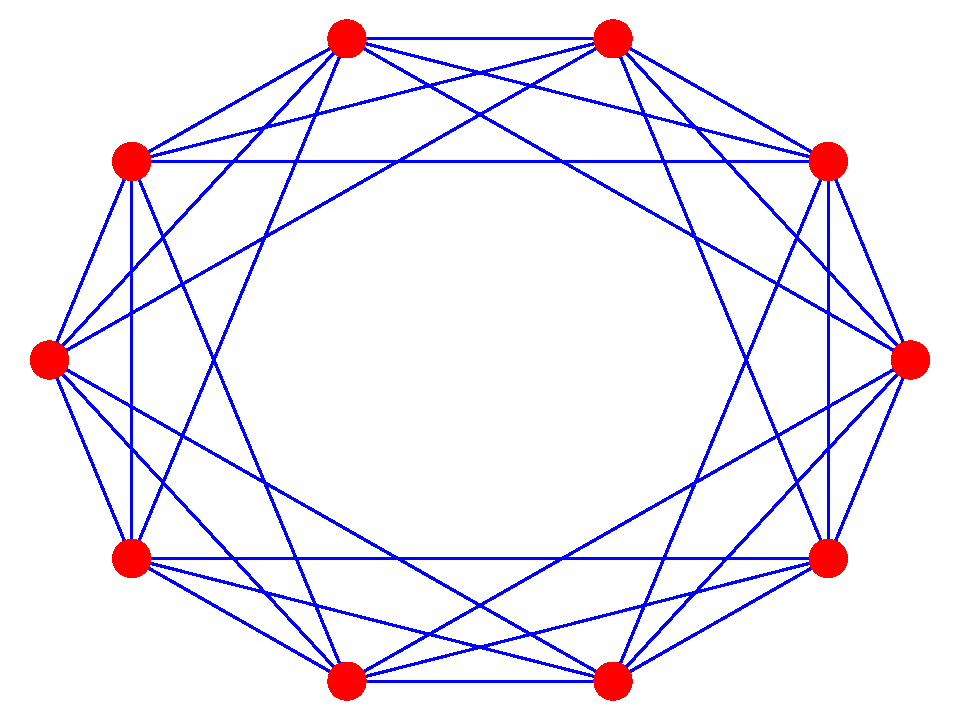
\includegraphics[trim={0 0 0 0},clip, scale=0.9]{n10k3.pdf}
    \caption{n=10, k=3}
    \label{fig:figure-4}
\end{figure}

\begin{figure}[h]
    \centering
    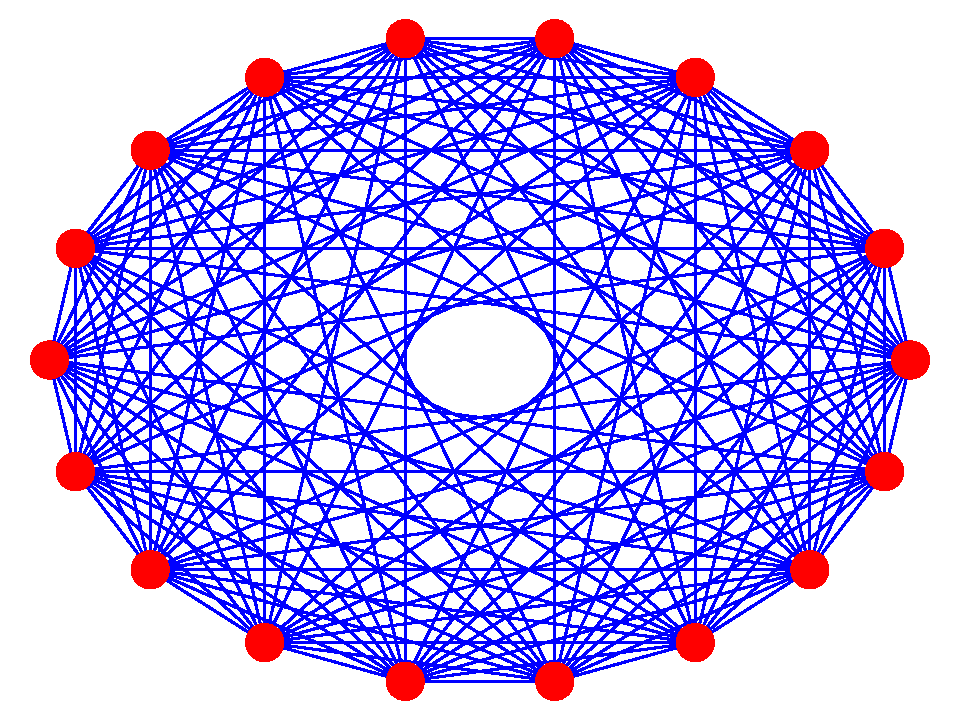
\includegraphics[trim={0 0 0 0},clip, scale=0.9]{n18k8.pdf}
    \caption{n=18, k=8}
    \label{fig:figure-4}
\end{figure}

\begin{figure}[h]
    \centering
    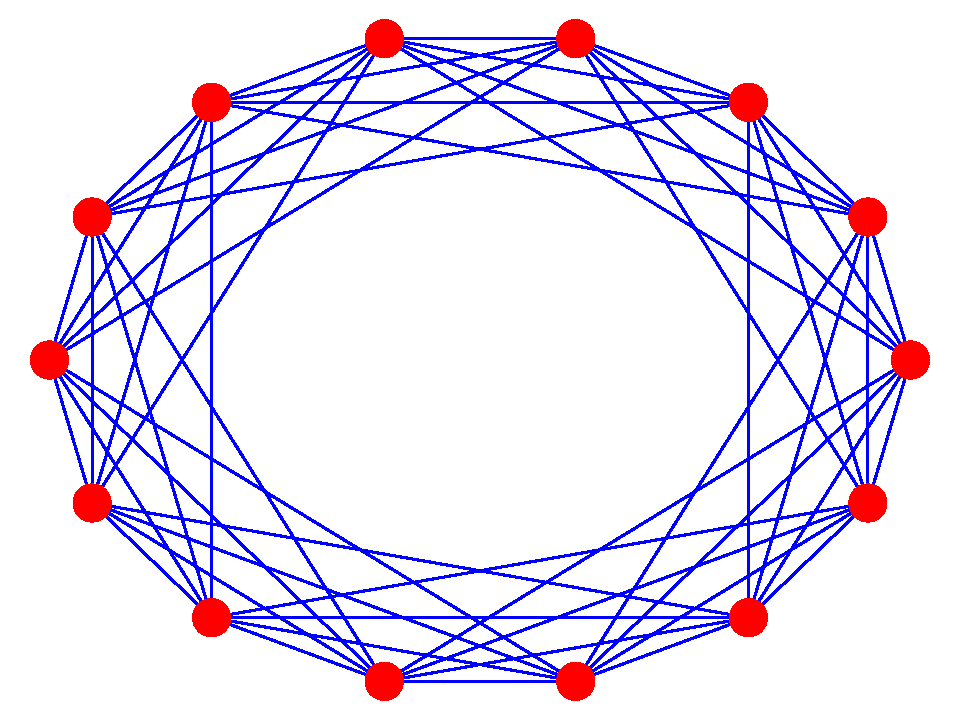
\includegraphics[trim={0 0 0 0},clip, scale=0.9]{n14k4.pdf}
    \caption{n=14, k=4}
    \label{fig:figure-4}
\end{figure}

\begin{figure}[h]
    \centering
    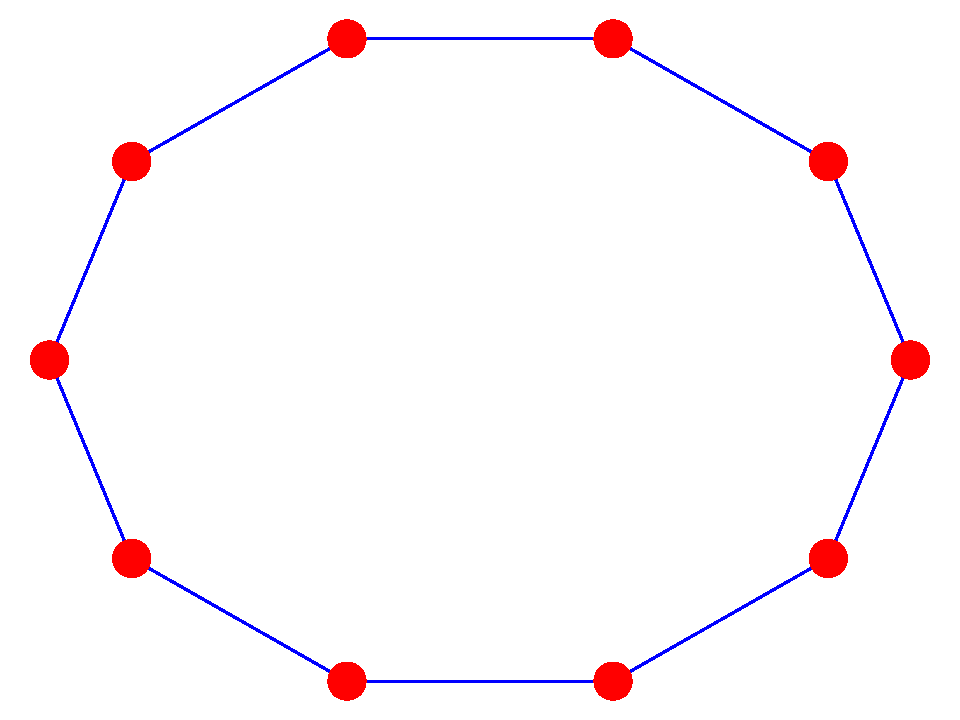
\includegraphics[trim={0 0 0 0},clip, scale=0.9]{n10k1.pdf}
    \caption{n=10, k=1}
    \label{fig:figure-4}
\end{figure}

\end{document}
\grid
\grid